
\chapter{Curves, Coordinates, and Differentials}

This chapter covers the following ideas. 


\begin{enumerate}

\item Model motion in the plane using parametric equations. In particular, how do you describe circles, ellipses, and lines using parametric equations.
\item Be able to convert between rectangular and polar coordinates. 
\item Graph polar functions in the plane. Find intersections of polar equations, and illustrate that not every intersection can be obtained algebraically (you may have to graph the curves).
\item Find derivatives, tangent lines, area, arc length, and surface area using parametric and polar equations.

\end{enumerate}


%%% Local Variables: 
%%% mode: latex
%%% TeX-master: "../multivariable-calculus"
%%% End: 




\section{Parametric Equations}

How can we describe motion in the plane?  One idea is to let $t$ represent time, and then write two equations $x=f(t),y=g(t)$ to describe the $(x,y)$ location of the point at any time $t$.  This gives us our first example of a mathematical ``function'' where we put in one value $t$ and get out two values $x$ and $y$.  This approach gives us a valuable way to study motion in the plane. The equations $x(t), y(t)$ are called parametric equations of a curve.

The parametric equations $x = \cos t, y=\sin t$ for $0\leq t\leq 2\pi$ describe motion along a circle of radius 1 in the plane.  You can convince yourself of this by plotting the points for various values of $t$ (make a $t,x,y$ table and start plotting points).  Alternatively, if you recall that $\cos^2 t+\sin^2 t = 1$, then you can replace $\cos t$ with $x$ and $\sin t$ with $y$ to obtain $x^2+y^2=1$, a Cartesian equation for a circle of radius 1.  Similarly you can show that $x=a\cos t, y=b\sin t$ for $0\leq t\leq 2\pi$ gives equations for an ellipse of the form $\frac{x^2}{a^2}+\frac{y^2}{b^2}=1$.  The graph of a function of the form $y=f(x)$ can always be written parametrically as $x=t,y=f(t)$, and then any equation we studied in first semester calculus can be analyzed using parametric equations. Using the identity $\cosh^2 x-\sinh^2 x =1$, the parametric equations $x=\cosh t,y=\sinh t$ give parametric equations for a hyperbola $x^2-y^2=1$, where $-\infty<t<\infty$. Because $\cosh x$ and $\sinh x$ trace out a hyperbola as parametric equations, they are called the hyperbolic trigonometric functions.  

To parametrize the line segment from $(1,2)$ to $(2,3)$, let's start by giving a Cartesian equation. The slope is $1/2$, so an equation is $y-2=\frac{1}{2}(x-1)$.  One option is to let $x=t$ and then $y=2+\frac{1}{2}(t-1)$. In this case, to get the curve to start at $x=1$ and end at $x=2$, we require $1\leq t\leq 2$. Another option is to let $t=\frac{1}{2}(x-1)$ or $x=1+2t$, and then $y-2=t$ or $y=2+t$. When $x=1$ we have $t=0$, and when $x=2$ we have $t=1/2$, so we require $0\leq t\leq 1/2$. There are infinitely many ways to parametrize the same curve.

We need to learn how to write parametric equations given a curve, and we need to learn how to find a Cartesian equation (remove $t$ from the equations) when we are given parametric equations.  In the textbook in 10.2, they give an example of the cycloid which leads to parametric equations. It is not crucial that you master the ideas behind a cycloid, rather that you learn how to parametrize curves. We will practice this idea in class all semester long. Obtaining a skill in parameterizing curves requires lots of practice. 

\subsection{Derivatives and Tangent lines}
How do you find the slope $\frac{dy}{dx}$ for a parametric curve?  The simple answer comes from the chain rule and essentially can be thought of as divide the top and bottom by $dt$, giving $\frac{dy}{dx} = \frac{dy/dt}{dx/dt}$. In other words, the derivative with respect to $x$ is found by dividing derivatives with respect to $t$.  This allows us to find tangent lines and more.  To find the second derivative $\frac{d^2y}{dx^2}$, we first find $dy/dx$ and then compute $d(dy/dx)/dt$ and divide it by $dx/dt$, namely 
$\ds \frac{d(\frac{dy}{dx})}{dx} = \frac{d(\frac{dy}{dx})/dt}{dx/dt}$ 
(again divide the top and bottom by $dt$). Often times people use dots to denote derivatives with respect to $t$, so we could write this as $dy/dx=\dot y/\dot x$.

As an example, consider the ellipse $x=\cos t, y=\sin t$. The derivatives with respect to $t$ are $\dot x = dx/dt = -\sin t$ and $\dot y= dy/dt=\cos t$. The derivative of $y$ with respect to $x$ is $dy/dx = \dot y/\dot x = \frac{\cos t}{-\sin t} = -\cot t$.  The derivative of $y'$ with respect to $t$ is $(-\cot t)' = \csc^2 t$. Dividing this by $\dot x = -\sin t$ gives $d^2y/dx^2 = \csc^3t$.  To find the tangent line to the curve at $t=\pi$, we compute  $x=\sqrt 2/2, y=\sqrt 2/2$, and $dy/dx = -\cot (\pi/4) = -1$. Using the point-slope form of a line, we have the tangent line as $(y-\sqrt 2/2) = -1 (x-\sqrt 2 /2)$.



\section{Polar Coordinates}

We now introduce a new coordinate system, the polar coordinate system.  This is just another way of referencing points in the plane.  We use {$r$ and {$\theta$ to reference points.  The distance from the origin to the point {$P$ is called {$r$, and the angle made by the positive {$ x $-axis and a ray from the origin through {$ P $ is called {$ \theta $.  The key equations $ x=r\cos\theta, y=r\sin\theta , x^2+y^2=r^2$ come directly from a right triangle with one vertex at the origin, another at the point $P$, and another directly above or below $P$ on the $x$-axis. 

The point $(r,\theta) =(2, \pi/2)$ represents the point $(x,y)=(0,2)$. The point $(r,\theta) =(3, \pi/4)$ represents the point $(x,y)=(3\frac{\sqrt{2}}{2},3\frac{\sqrt{2}}{2})$. Notice that the point $(1,\pi)$ in polar coordinates is the same as the point $(1,3\pi)$ or $(-1,-\pi)$ in polar coordinates.  The same $(x,y)$ point in the plane can be represented by infinitely many different polar coordinate pairs.
\subsection{Converting between polar and Cartesian coordinates and graphing}
The graph of $r=2$ is a circle of radius $2$ in the plane.  The graph of $\theta =  \pi/3$ is a straight line through the origin with angle of inclination $\pi/3$.  The line $x=4$ can be rewritten in polar coordinates as $r\cos\theta = 4$, or $r=4\sec\theta$.  The polar coordinate equation $r=2\sin\theta $ can be converted to rectangular coordinates by multiplying both sides by $r$, giving $r^2 = 2r\sin\theta$, and then using the key equations to obtain $x^2+y^2 = 2y$, which is the equation of a circle $x^2+y^2-2y+1=1$, or $x^2+(y-1)^2=1$ centered at $(0,1)$ of radius $1$ (I completed the square to complete this example). The key equations will allow you to convert from one system to another. You may need to multiply both sides of an equation by $r$ to do a conversion (as in the last example).

To plot a polar equation, we just make an $r,\theta, x,y$ table and start plotting points.  You will discover after some practice that there are symmetries that you can use to help you learn how to plot polar curves.  To plot the curves by hand, try putting in values of $\theta$ which are on the unit circle, in particular use $0,\pi/2,\pi,3\pi/2$.  When you connect dots on your graphs, realize that you wrap around counter-clockwise as theta increases, and the variable $r$ that is changing is the distance from the origin.  Some common curves are shown below:

\newcommand{\mywidth}{1.3in}
\begin{center}
\begin{tabular}{cccc}
%polar_plot(cos(3*x),(x,0,2*pi),color='black',aspect_ratio=1).save('rose.pdf',aspect_ratio=1)
%polar_plot(2*cos(x)+1,(x,0,2*pi),color='black',aspect_ratio=1).save('limacon.pdf',aspect_ratio=1)
%polar_plot(1-cos(x),(x,0,2*pi),color='black',aspect_ratio=1).save('cardioid.pdf',aspect_ratio=1)

% cosines = [cos(-pi/2+pi*i/100) for i in range(201)]
% v = [(1/c, tan(-pi/2+pi*i/100)) for i,c in enumerate(cosines) if c != 0]
% L = [(a/(a^2+b^2), b/(a^2+b^2)) for a,b in v]
% p = line(L, color='black')
% p.save('lemniscate.pdf',aspect_ratio=1)

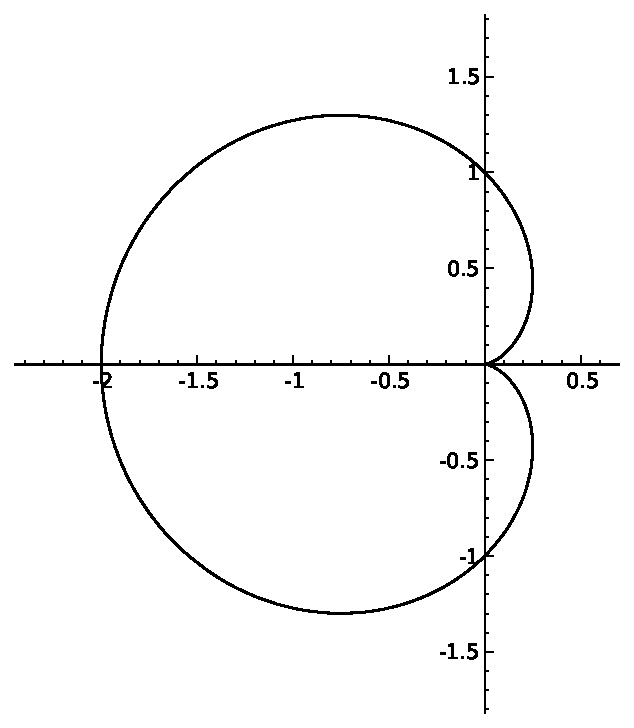
\includegraphics[width=\mywidth]{01-Curves-Coordinates-Differentials/cardioid}&
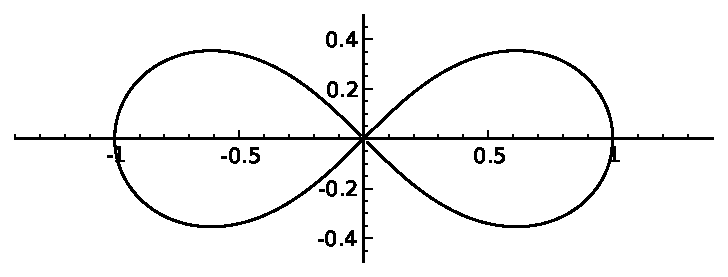
\includegraphics[width=\mywidth]{01-Curves-Coordinates-Differentials/lemniscate}&
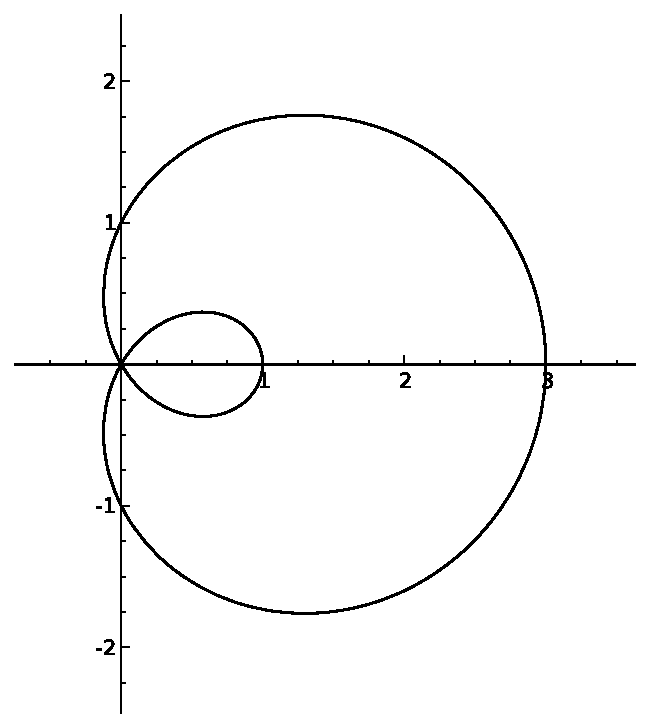
\includegraphics[width=\mywidth]{01-Curves-Coordinates-Differentials/limacon}&
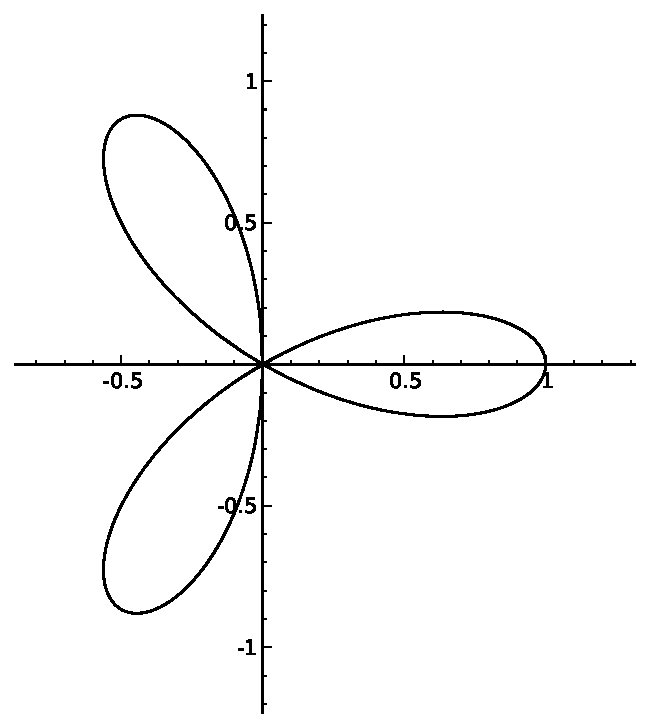
\includegraphics[width=\mywidth]{01-Curves-Coordinates-Differentials/rose}
\\
Cardioid&
Lemniscate&
Limacon&
Rose
\\
$r=1-\cos\theta$&
$r^2=\sin 2\theta$&
$r=2\cos\theta+1$&
$r=\cos 3\theta$
\end{tabular}
\end{center}

\subsection{Finding Intersections}
One problem with finding the intersection of two polar graphs is that there are many ways to represent the same point in polar coordinates.  Hence, when you solve for the intersection of two polar graphs, you may not find all the intersection points algebraically. Often you must graph the polar curves in addition to finding the points of intersection.  For example, the two curves $r=1-\cos\theta$ (a cardioid) and $r=\cos\theta$ (a circle of radius 1/2 centered at (1/2,0)) intersect in three points.  Solving for $\theta$ we have $\cos\theta = 1-\cos\theta$, or $2\cos\theta = 1$, or $\cos\theta = \frac{1}{2}$.  This occurs when $\theta = \pm \frac{\pi}{3}$. Hence the two points of intersection are $(x,y)=(r\cos\theta,r\sin\theta) = (1/4,\pm\sqrt 3 / 4)$.  The algebraic solution misses completely the fact that $(x,y)=(0,0)$ is an intersection point of the two graphs. It is best to graph any polar curves when you wish to find their intersection.



\section{Calculus and Differentials}

\subsection{Slope}
If a curve is given parametrically as $x=f(t),y=g(t)$, then we can find $\ds\frac{dy}{dx}$ using the chain rule. Symbolically we just divide both $dx$ and $dy$ by $dt$, and obtain $\ds\frac{dy}{dx} = \ds\frac{dy/dt}{dx/dt}$.  For example, if $x=3t$ and $y=t^2-t$, then $\ds\frac{dy}{dx} = \ds\frac{dy/dt}{dx/dt}=\frac{2t-1}{3t}$.  This is how we find the slope of graphs of parametric curves.

If the curve is given by a polar coordinate equation $r(\theta)=f(\theta)$, then we use the same principle.  Recall $x=r\cos\theta = f(\theta)\cos\theta$ and $y=r\sin\theta = f(\theta)\sin\theta$.  Hence we have 
$\ds\frac{dy}{dx} 
= \ds\frac{dy/d\theta}{dx/d\theta} 
= \frac{\frac{d}{d\theta} f(\theta)\sin\theta }{\frac{d}{d\theta} f(\theta)\cos\theta } 
= \frac{f^\prime (\theta)\sin\theta +f(\theta)\cos\theta }{ f^\prime(\theta)\cos\theta - f(\theta)\sin\theta} 
$. Don't worry about memorizing this formula, rather realize that it is just $\ds\frac{dy/d\theta}{dx/d\theta}$.





\subsection{Area Differential $dA$}

To find the area swept out by a segment from the origin to a polar curve, we first need to recall that the area of a sector of a circle is $\displaystyle \frac 12 r^2 \theta$. To derive this, just recall the area of a circle is  $\pi r^2$. So half a circle has area $\displaystyle \frac{\pi}{2}r^2$. If you sweep out $\theta$ radians, then you have covered $\displaystyle \frac{\theta}{2\pi}$ percent of the circle. So the area covered is $\displaystyle \frac{\theta}{2\pi}\cdot \pi r^2$.  

Now we take the simple formula, $\displaystyle \frac 12 r^2 \theta$ and use it to derive the integral formula $ \int_\alpha^\beta \frac 12 r^2 d\theta.$ Consider the region swept out by a segment from the origin to the polar curve $r=f(\theta)$ as $\theta$ ranges from $\alpha$ to $\beta$. Break up the region into small sectors, each having interior angle $\Delta \theta$. By making $\Delta \theta$ small enough, we can approximate the area $\Delta A_i$ of each sector by assuming the radius is constant, $f(\theta_i)$.  This gives $\Delta A_i\approx \frac12 f(\theta_i)^2 \Delta \theta$. To find the total area, we add up all the little areas and take a limit as $\Delta \theta\to 0$, as follows: $$A = \lim_{\Delta \theta\to 0} \sum\Delta A_i
=\lim_{\Delta \theta\to 0} \sum\frac12 f(\theta_i)\Delta \theta
=\int_\alpha^\beta \frac12 f(\theta)^2d \theta
=\int_\alpha^\beta \frac12 r^2d \theta.
$$
We use the differential notation 
$dA=\frac{1}{2}r^2d\theta$ to remember the integration formula.  If you can remember the area of a sector of a circle, then you can remember the integration formula.  You probably recall already the differential notation
$dA=f(x)dx$
To find area, all you have to do is remember that area is the integral of the area differential $dA$, so $A=\int dA = \int_a^b f(x)dx = \int_\alpha^\beta\frac{1}{2}r^2d\theta. $ To find area between two polar curves, just find the area inside the outer curve, and subtract the area inside the inner curve. The area inside the cardioid $r=1-\cos\theta$ is given by $\int_0^{2\pi}\frac{1}{2}(1-\cos\theta)^2d\theta$, which we would let a computer calculate for us.
 
\subsection{Arc Length Differential $ds$}


Finding length ({$\Delta s$}) along a straight line is done by finding the change in {$x$} (called {$\Delta x$}) and the change in {$y$} ({$\Delta y$}), and then using the Pythagorean identity to get {$\Delta s = \sqrt{\Delta x^2+\Delta y^2}$}. If a curve is not straight, then start by breaking the curve up into a bunch of small pieces of length {$\Delta s_i$}.  Along each small piece, the curve is approximately straight, so we approximate each {$\Delta s_i$} with {$\sqrt{\Delta x_i^2+\Delta y_i^2}$}. In differential notation this becomes $ds = \sqrt{dx^2+dy^2}$.  To find arc length {$s$}, we add up ({$\sum ds$}) the little pieces of arc length and take a limit to get {$s = \int_C ds = \int_C\sqrt{dx^2+dy^2}$}.  For a function $y=f(x), a\leq x\leq b$ whose independent variable is $x$, you can multiply $ds$ by $1=\frac{dx}{dx}$ to obtain $ ds = \sqrt{dx^2+dy^2}\frac{dx}{dx} = \sqrt{\left(\frac{dx}{dx}\right)^2+\left(\frac{dy}{dx}\right)^2}dt=\sqrt{1+\left(\frac{dy}{dx}\right)^2}dt$ which means arc length is $ s=\int_C ds = \int_a^b \sqrt{1+\left(\frac{dy}{dx}\right)^2}dx$. Similarly, for $x=g(y), c\leq y\leq d$ we multiply by $\frac{dy}{dy}$ to obtain
$ \int_c^d \sqrt{\left(\frac{dx}{dy}\right)^2+1}dy$. For 
parametric equations $x(t),y(t), a\leq t\leq b$ we multiply by $\frac{dt}{dt}$ to obtain $ \int_a^b \sqrt{\left(\frac{dx}{dt}\right)^2+\left(\frac{dy}{dt}\right)^2}dt$. 
The polar coordinate version $\int_\alpha^\beta \sqrt{r^2+\left(\frac{dr}{d\theta}\right)^2}d\theta$ comes from the nontrivial simplification $\left(\frac{dx}{d\theta}\right)^2+\left(\frac{dy}{d\theta}\right)^2 = r^2+\left(\frac{dr}{d\theta}\right)^2$, where $x=r\cos \theta, y=r \sin\theta$. 
Hence, to find the arc length for parametric or polar curves, we just integrate the arc length differential.


\subsection{Surface Area Differential $d\sigma$ (of a surface of revolution)}
When you revolve a curve about a line, the radius of rotation is the distance to the line. We will now develop formulas for find the surface area of a surface of revolution given by rotating about a line. 

Start by breaking the curve up into small pieces (as done before). The length of each piece is approximately given by the arc length approximate {$\Delta s_i$, which is a straight line segment from one end of the small portion of the curve to the other. We assume that the radius is constant, namely the distance {$radius_i$ to the line. 
If we rotate about the $x$-axis, then $radius_i=y_i$.  
If we rotate about the $y$-axis, then $radius_i=x_i$.
The surface area of a frustrum of a cone is $\Delta \sigma_i = 2\pi radius_i \Delta s_i$ (we use $\sigma$ to designate surface area). Adding each small pieces of surface area up $\sigma=\displaystyle \sum \Delta\sigma_i$, we get the integration formulas $\displaystyle
\sigma = \int d\sigma
= \int 2\pi\ radius\ ds
= \int_a^b 2\pi\ radius\ \sqrt{\left(\frac{dx}{dt}\right)^2+\left(\frac{dy}{dt}\right)^2}dt
= \int_\alpha^\beta 2\pi\ radius\ \sqrt{r^2+\left(\frac{dr}{d\theta}\right)^2}d\theta
.$
Note that if you can remember $d\sigma = 2\pi\ radius\ ds,$
then you just have to know what the radius is, and what to use for $ds$.  


The surface area of a surface of revolution formed by revolving a polar curve about the $x$-axis is given by the formula  $\ds \int_\alpha^\beta 2\pi |y| ds =
\int_\alpha^\beta 2\pi r\sin\theta \sqrt{r^2+\left(\frac{dr}{d\theta}\right)^2}d\theta$, provided $y\geq 0$.
When we revolve about the $y$-axis we obtain instead the formula 
$\ds \int_\alpha^\beta 2\pi |x| ds=
\int_\alpha^\beta 2\pi r\cos\theta \sqrt{r^2+\left(\frac{dr}{d\theta}\right)^2}d\theta$, provided $x\geq 0$.

If we rotate about a line such as $x=3$, then the distance to the line $x=3$ is given by $|x-3|$, so our formula is  $\ds \int_\alpha^\beta 2\pi |x-3| ds =
\int_\alpha^\beta 2\pi (r\cos\theta -3) \sqrt{r^2+\left(\frac{dr}{d\theta}\right)^2}d\theta$, provided $x\geq 3$ (otherwise we just leave the absolute values in the problem).

%%% Local Variables: 
%%% mode: latex
%%% TeX-master: "../multivariable-calculus"
%%% End: 





